%Autor: Simon Walker
%Version: 1.0
%Datum: 25.06.2020
%Lizenz: CC BY-NC-SA


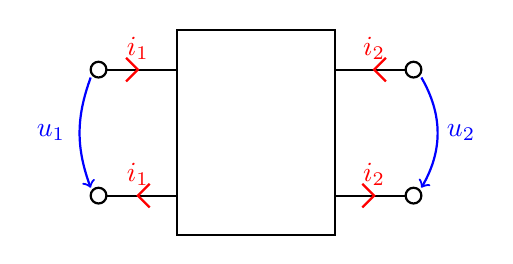
\begin{tikzpicture}

%Symbol
\draw[thick] (-1, -1.3) rectangle (1, 1.3);
\draw[thick] (-1,0.8) -- (-2,0.8);
\draw[thick, fill=white] (-2,0.8) circle (0.1);
\draw[thick] (-1,-0.8) -- (-2,-0.8);
\draw[thick, fill=white] (-2,-0.8) circle (0.1);

\draw[thick] (1,0.8) -- (2,0.8);
\draw[thick, fill=white] (2,0.8) circle (0.1);
\draw[thick] (1,-0.8) -- (2,-0.8);
\draw[thick, fill=white] (2,-0.8) circle (0.1);

%Strompfeile
\draw[red, thick] (-1.5, 0.8) node[above, red] {$i_1$} ++(-0.15, 0.15) -- ++(0.15, -0.15) -- ++(-0.15, -0.15);
\draw[red, thick] (-1.5, -0.8) node[above, red] {$i_1$} ++(0.15, 0.15) -- ++(-0.15, -0.15) -- ++(0.15, -0.15);

\draw[red, thick] (1.5, 0.8) node[above, red] {$i_2$} ++(0.15, 0.15) -- ++(-0.15, -0.15) -- ++(0.15, -0.15);
\draw[red, thick] (1.5, -0.8) node[above, red] {$i_2$} ++(-0.15, 0.15) -- ++(0.15, -0.15) -- ++(-0.15, -0.15);

%Spannungspfeile
\draw[blue, ->, thick, out=-110, in=110] (-2.1, 0.7) to (-2.1, -0.7);
\node[left, blue] at (-2.3,0){$u_1$};

\draw[blue, ->, thick, out=-60, in=60] (2.1, 0.7) to (2.1, -0.7);
\node[right, blue] at (2.3,0){$u_2$};


\end{tikzpicture}
